\documentclass[twocolumn]{article}

\usepackage{IJCISIM,multicol,times}

\usepackage{epsfig}
\usepackage[utf8]{inputenc}
\usepackage{graphicx}
\usepackage[T1]{fontenc}
\usepackage[hyphens]{url}
\usepackage{listings}
%\usepackage{hyperref}
\def\sectionautorefname{Section}
\usepackage{textcomp}
\lstset{
        basicstyle=\ttfamily\scriptsize,
        upquote=true,
        showspaces=false,
        showstringspaces=false,
        showtabs=false,
        tabsize=2,
        frame=none,
        breaklines,
        numbers=none,
        framexleftmargin=2mm,
        xleftmargin=2mm,
}

% todo macro
\usepackage{color}
\newcommand{\todo}[1]{\noindent\textcolor{red}{{\bf \{TODO}: #1{\bf \}}}}

%% Define a new 'smallurl' style for the package that will use a smaller font.
\makeatletter
\def\url@smallurlstyle{%
  \@ifundefined{selectfont}{\def\UrlFont{\sf}}{\def\UrlFont{\scriptsize\ttfamily}}}
\makeatother
%% Now actually use the newly defined style.
\urlstyle{smallurl}
\newcommand{\nofootnote}[1]{~#1}

% correct bad hyphenation here
\hyphenation{op-tical net-works semi-conduc-tor}


\parindent0pt


\begin{document}
\pagestyle{empty}
\sloppy


\title{Adding Meaning to Social Network Microposts\\ via Multiple Named Entity Disambiguation APIs\\ and Tracking Their Data Provenance}

\author{\bf Thomas Steiner$^1$, Ruben Verborgh$^2$, Joaquim Gabarro$^1$, and Rik Van de Walle$^2$\\[1em]
$^1$Universitat Polit\`ecnica de Catalunya,
Department LSI,
08034 Barcelona, Spain\\
\textit{\{tsteiner, gabarro\}@lsi.upc.edu}\\[1em]
$^2$Ghent University -- IBBT,
ELIS -- Multimedia Lab,
B-9050 Ledeberg-Ghent, Belgium\\
\textit{\{ruben.verborgh, rik.vandewalle\}@ugent.be}}

\maketitle

\begin{abstract}
Social networking sites such as Facebook, Twitter, or Google+ let their users  create microposts directed to all, or a subset of their contacts. Users can respond to microposts, or in addition to that, also click a \textit{Like}, \textit{+1}, or \textit{ReTweet} button to show their appreciation for a certain micropost. Adding semantic meaning in the sense of \emph{unambiguous intended ideas} to such microposts can, for example, be achieved via Natural Language Processing (NLP) and named entity disambiguation. Therefore, we have implemented a mash-up NLP API, which is based on a combination of several third party NLP APIs in order to retrieve more accurate results in the sense of emergence. In consequence, our API uses third party APIs opaquely in the background in order to deliver its output. In this paper, we describe how one can keep track of data provenance and credit back the contributions of each single API to the joint result of the combined mash-up API. In addition to that, we show how the existence of provenance metadata can help understand the way a combined result is formed, and optimize the result combination process. Therefore, we use the HTTP Vocabulary in RDF and the Provenance Vocabulary.
\end{abstract}

\keywords{social networks, data provenance, web services, named entity disambiguation, named entity consolidation}

\section{Introduction}                                                      \label{sec:introduction}
According to official Facebook statistics~\cite{Facebook}, the social networking website has more than 500 million active users out of which half log on to Facebook in any given day. The average Facebook user has 130 friends, and creates 90 pieces of content each month. This sums up to the impressive number of overall twenty-two billion five hundred million pieces of content per month. Similar to the microblogging website Twitter with its full text Twitter search\footnote{\texttt{https://search.twitter.com/}}, Facebook as well offers both a search feature on the website, and a JSON-based search API over status updates from all global Facebook members\footnote{Facebook search for \textit{salamanca, spain}: \texttt{http://bit.ly/ogpsearch}}. In order to perform data mining, a statistically significant amount of microposts is necessary (this is also known as access to the ``firehose''). However, while Twitter grants selected parties access to its Streaming API~\cite{Twitter} for research purposes, for Facebook there is no such documented option. To address this shortage, we have developed browser extensions called Facebook Swarm NLP\footnote{\texttt{http://bit.ly/facebookswarmnlp}} and Twitter Swarm NLP\footnote{\texttt{http://bit.ly/twitterswarmnlp}} for the Google Chrome Web browser. These extensions inject JavaScript code into the Facebook.com or Twitter.com homepages to perform data analysis on the encountered set of microposts by sending the results to a central data processing point. Therefore, the extensions first check if the user is logged in to Facebook or Twitter, and if so, retrieve all status updates from the contacts that are displayed on the current user's timeline. Second, the extensions perform named entity extraction and disambiguation via Natural Language Processing (NLP) using a remote NLP API on each of the microposts in order to add semantic meaning to them. The extracted named entities are then displayed below each micropost, as illustrated in Figure~\ref{fig:facebook}. Finally the extracted named entities are sent to a central Web analytics~\cite{Kaushik} framework to compute basic or advanced trends, for example by ranking the most discussed-about named entities per day, or by pivoting named entities by Web analytics data, like users' geographic locations.

\begin{figure}[htb!]
  \centering
    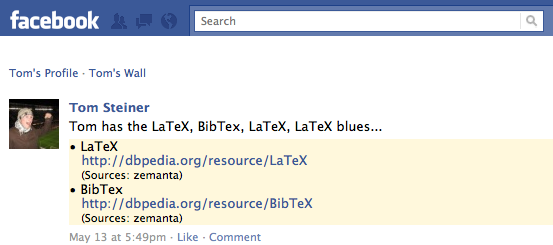
\includegraphics[width=0.45\textwidth]{facebook-swarm-nlp.png}
  \caption{Facebook Swarm NLP browser extension. Extracted named entities have a pale yellow background.}     
  \label{fig:facebook}
\end{figure}

As mentioned before, in order to perform named entity extraction and disambiguation, we rely on a mash-up API that calls existing third party NLP APIs in the background and that delivers the combined results of these APIs in a consolidated way. It is  desirable (i)~to credit back the contribution of each single third party API to the joint results, and (ii)~to track the provenance of the joint results in order to understand how they were formed. We will show at the concrete example of the mash-up NLP API used for our browser extension how these two constraints can be fulfilled in a generalizable way.

The remainder of this paper is structured as follows: we discuss related work in Section~\ref{sec:related}. In Section~\ref{sec:services}, we introduce APIs that allow for unstructured data to be converted into Linked Data. In Section~\ref{sec:tracking}, we describe how we automatically maintain provenance metadata in our API. Section~\ref{sec:future} presents future work. Finally Section~\ref{sec:conclusion} ends the paper with a conclusion. \todo{Fix}

\section{Related Work}\label{sec:related}
Named entity disambiguation or mapping is not only a major challenge of research in the Semantic Web world, but also in 
Natural Language Processing. In the following, we present representative related work around this task, categorized by
different approach classes. 

\subsection{Entity Disambiguation Using Lexical Databases}

In \cite{Choudhury:YouTube} Choudhury et al. describe a framework for semantic enrichment, ranking, and integration of
Web video tags using Semantic Web technologies. In order to enrich the oftentimes sparse user-generated tag space, meta
data like the recording time and location, or the video title and video description are used, but also social features
such as playlists where a video appears in and related videos. Next, the tags are ranked by their co-occurrence and in
a final step interlinked to DBpedia\footnote{\url{http://dbpedia.org/}} concepts for greater integration with other
datasets. Choudhury et al. disambiguate the tags based on WordNet\cite{Princeton:WordNet} synsets if possible (i.e., if
there is only one matching synset in WordNet, the corresponding WordNet URI in DBpedia is selected. If there are more
than one matching synsets, the tags and their context tags similarity is computed and thereby tried to decide on an
already existing tag URI). For words that are not contained in WordNet, Sindice\footnote{\url{http://sindice.com/}} is
used to find the most probable concept.

\subsection{Entity Disambiguation Using Semantic Coherence And News Trends}

In \cite{Fernandez:IdentityRank} Fern\'{a}ndez et al. examine entity disambiguation in the context of news annotation.
They introduce a novel algorithmic approach to entity disambiguation called \textit{IdentityRank}. Running IdentityRank
on a news item consists of three steps: finding the candidate instances in the news ontology for each entity in the
news item, ranking these candidate instances using a modified version of PageRank\cite{Brin:PageRank}, and finally
retraining the algorithm with the journalist's feedback once the process is finished. IdentityRank first takes into
account the number of occurrences of candidate entities in the past in order to find news trends, and second the
occurrences of candidate entites in past articles in the same categories in order to find semantic coherences (for
example, the name of a soccer player will most probably be mentioned in past articles categorized as sports-related).

\subsection{Entity Disambiguation Using Disambiguation Dictionaries}

In \cite{Nguyen:NamedEntity} Nguyen et al. show how disambiguation dictionaries can be used to disambiguate entities
using disambiguation data extracted from Wikipedia\footnote{\url{http://wikipedia.org/}}, mostly based on special
disambiguation pages\footnote{E.g., \url{http://en.wikipedia.org/wiki/Oolong_(disambiguation)}}. For a set of entity
candidates, all disambiguations are ranked using the well-known TF-IDF (or cosine similarity) method from the field of
information retrieval. The approach is a hybrid and incremental process that utilizes previously identified named
entities and related terms co-occurring with ambiguous names in a text for entity disambiguation.

\subsection{Entity Disambiguation Using Corpusses}

Cucerzan shows in \cite{Cucerzan:Wikipedia} the use of a corpus like Wikipedia for entity disambguation. The
surrounding words of the to-be-disambiguated terms plus the tags and categories of the related Wikipedia articles are
then used to determine semantic coherence and thus to decide on the most probable entity candidate. This happens
through a process of heuristically maximizing the agreement between contextual information extracted from Wikipedia and
the context of a document.

\subsection{Entity Disambiguation Using Search Query Logs}

In \cite{Billerbeck:QueryLogs} Billerbeck et al. use click graphs and session graphs of users' search engine sessions
to semantically bridge different queries in order to retrieve entities for a concrete entity retrieval query. Click
graphs are created by using queries and URLs as nodes and connecting and weighting them by their user click
frequencies, and session graphs by using only queries as nodes with edges between them if they appear in the same user
sessions, again weighted by co-occurrence frequencies. An exemplary entity retrieval query might be \textit{hybrid
cars}, semantically bridgeable queries might be \textit{toyota prius}, or \textit{honda civic hybrid}). These entities
are then ranked and returned to the user.

\subsection{Combining Different Web Services}
In~\cite{Groth:2009:MPD:1462159.1462162}, Groth et al. describe how through tools and technologies such as Yahoo Pipes, Really Simple Syndication (RSS) and APIs, so-called mash-ups can be created in a dynamic, just-in-time way, combining data from different data sources. The authors are driven by the motivation to allow for trust and confidence in mash-ups, and therefore consider it critical to be able to analyze the origin of combined results. They suggest an approach based on OWL and XML, with a focus on process documentation. However, different from us, where the goal is to transparently add provenance data at API invocation level, their focus is more on overall process documentation in the context of a mash-up application.

The focus of Carroll et al. in~\cite{carroll2005} is on the provenance of triples in the Semantic Web world, namely, for making statements about triples in graphs. Therefore, the paper introduces the concept of named graphs, an extension to RDF. In contrast to our work, Carroll et al. focus purely on using triples to make statements about triples (that is, they stay in the RDF world), whereas our approach uses RDF to make statements about potentially any API result. That is, our approach is not limited to RDF results, albeit in the concrete case we use RDF in addition to JSON as API result.
 
In the WS-* world, BPEL4WS, described by Curbera et al. in~\cite{Curbera:2003:NSW:944217.944234} provides a formal language for the specification of business processes and business interaction protocols. This allows for the combination of several APIs, however, it does not credit back concrete outputs of a combined API to the underlying APIs.

\section{Structuring Unstructured Textual Data}
When we speak of adding structure to unstructured textual data we mean the process of extracting the main concepts in the form of named entities from a given text. An ``entity" is defined\footnote{\url{http://wordnetweb.princeton.edu/perl/webwn?s=entity}} by WordNet as ``that which is perceived or known or inferred to have its own distinct existence (living or nonliving)". Typically named entities from a text can be persons, companies, organizations, geographies, but also things like quantities, expressions of time, books, albums, authors etc. The extraction is based on Natural Language Processing (NLP) and Machine Learning.

\subsection{Natural Language Processing Services}\label{sec:nlp-services}
Natural Language Processing is defined\footnote{\url{http://wordnetweb.princeton.edu/perl/webwn?s=natural\%20language\%20processing}} as ``the branch of information science that deals with natural language information". From the many NLP toolkits, in the following we list some NLP Web services that link to datasets in the LOD cloud described in Section~\ref{sec:lodcloud} in order to disambiguate named entities.

\subsubsection{OpenCalais}\label{sec:opencalais}
OpenCalais~\cite{OpenCalais} is the only Web service we use that provides details on occurrences in concrete sections of the submitted coherent text. This allows for exact matching of the location in the text where a certain entity is believed to appear. This is especially useful as OpenCalais is also oftentimes capable of recognizing references within the text to prior discovered entities (see the emphasized words as an example: ``\emph{Obama} thanked people for their work in ensuring the victory. \emph{He} also thanked his family […]"). An OpenCalais response consists of three parts:

\begin{itemize}
\item a list of overall topics that the text could be categorized in.
\item a list of concrete entities that occur in the text.
\item a list of social tags that a human being might assign to the text.
\end{itemize}

The problem with the extracted entities is that they are not always disambiguated. An example is the URI \url{http://d.opencalais.com/pershash-1/cf42394f-4ae9-3e8e-958a-088149c86565.html} that represents the concept of type ``person" of Barack Obama. However, president Barack Obama is also represented by the URI \url{http://d.opencalais.com/pershash-1/cfcf1aa2-de05-3939-a7d5-10c9c7b3e87b.html} that was returned in one and the same response to one of our test requests. A second issue is that only a tiny fraction of the returned entities link to other Linked Open Data (LOD) sources in the LOD cloud. In order to find links to the linking hub DBpedia, each returned entity has to be retrieved at the expense of an HTTP request, and the returned RDF has to be checked for said links.

\subsubsection{AlchemyAPI}
AlchemyAPI~\cite{AlchemyAPI} differentiates between entities and concepts, however, in practice the difference being very subtle, we can treat entities and concepts the same. Overall the AlchemyAPI results are very accurate and of mostly excellent Linked Data quality as there are links to well-known members of the LOD cloud, among others to DBpedia, OpenCyc, and Freebase. AlchemyAPI also provides links to other data sources, however, sometimes the returned URIs resolve to 404 ``Not found" errors (one example that we came across during our tests was the URI \url{http://umbel.org/umbel/ne/wikipedia/George_W._Bush.rdf}, which should represent the concept of the person George W. Bush). AlchemyAPI also oftentimes returns very related, but not directly relevant entities.

\subsubsection{Zemanta}
Zemanta~\cite{Zemanta} provides high quality entities that are linked to well-known members of the LOD cloud, e.g. DBpedia, Semantic CrunchBase, or Freebase. Zemanta convinces through very accurate entity disambiguation. We could not find any evident problem with the service, except for the sometimes relatively small number of entities, where the other services we use offer more.

\subsubsection{DBpedia Spotlight}
DBpedia Spotlight~\cite{spotlight} is a tool for annotating mentions of DBpedia resources in text, providing a solution for linking unstructured information sources to the Linked Open Data cloud through DBpedia. DBpedia Spotlight performs named entity extraction, including entity detection and disambiguation with adjustable precision and recall.

\section{Discussion Of Potential Entity Mapping Approaches}\label{sec:discussion}

For this section we recall our definition of \textit{entity mapping}: the process of mapping a string literal to the
most probable entity identified by a URI that represents said string literal. In consequence in the paragraph we
highlight some differences from the related work to our work.

\subsection{Differences Between Related Work And Our Approach}

The main difference between all previously mentioned approaches and our approach is that they make use of context
available in form of surronding words, document fragments, or even the whole document of a to-be-disambiguated term. In
contrast, we consider each term without any surrounding context. This obviously makes our main objective, besides
entity mapping \textit{per se}, judging entity disambiguation quality (or as we call it entity uncertainty) an almost
impossible task. This is why we bring search query logs from general search engines into play in order to potentially
put terms in an albeit limited context.

The first hypothesis behind our approach is that people of today's general search engines have learnt how to deal with
their imperfections. For example, if a user wishes to retrieve general information about German youngster soccer player
Thomas M\"{u}ller (both, \textit{thomas} and \textit{m\"{u}ller} being very common German first and last names), the
user knows that in order to perfectly disambiguate this query she needs to append a \textit{query refinement} like
\textit{soccer player} or \textit{bayern munich} to the name, so that the actual query is, e.g.,  \textit{thomas
m\"{u}ller soccer player}. Whereas for Argentinian ex-soccer player Diego Maradona, because of his world-wide
popularity (e.g., FIFA player of the century), a simple name-based query like \textit{diego maradona} is known by the
user to be sufficient.

Our second hypothesis is thus that for an ambigous term $t_{amb}$ there exists a certain quotient $q_{disamb}$ of
search queries such that

$$ q_{disamb} = \frac{n_{queries\; for\; {t_{amb}}}}{n_{queries\; for\; t_{amb}\; with\; query\; refinement\; t_{ref}}}
= \frac{n_{t_{amb}}}{n_{{t_{amb}\; t_{ref}}}}$$

A na\"{i}ve idea would be to assume that whenever $q_{disamb} > 0$ the term is disambigous (i.e., if more people search
for the term $t_{amb}$ alone than people search for the term $t_{amb}$ together with a query refinement $t_{ref}$).
However, in practice people oftentimes search more focused, for example, for \textit{diego maradona videos}. Part of
our hypothesis is thus that empirically a threshold for $q_{disamb} < 0$ can be determined that marks a term $t_{amb}$
as disambiguous, or not.

\subsection{Dealing With Entity Mapping Services}

In this section we motivate the use of multiple existing entity mapping Web services in parallel for the task of
obtaining entity candidates for a string literal. In addition to that we also introduce the notion of
\texttt{owl:sameAs}-based approaches.

Existing entity mapping Web services take as input parameter a string literal, and return a ranked list of entity
candidates, all identified by URIs, and enriched by depending on the service more or less meta information. In order to
gain confidence in a decision it is a common idea to rely not only on the response from one source, but to
independently request responses from several sources. Figure \ref{fig:diagram} illustrates this idea for four entity
mapping Web services. The figure has two levels: the direct result level that contains the direct output of the
particular entity mapping service, and the \texttt{owl:sameAs} level that contains \texttt{owl:sameAs} results for the
direct results. These are obtained either from data in the direct result entities themselves, or from a Web service
like sameAs.org\footnote{\url{http://sameas.org/}}, which is based on research from Glaser et al. in
\cite{Glaser:SameAs}.

\begin{figure*}
 \centering
 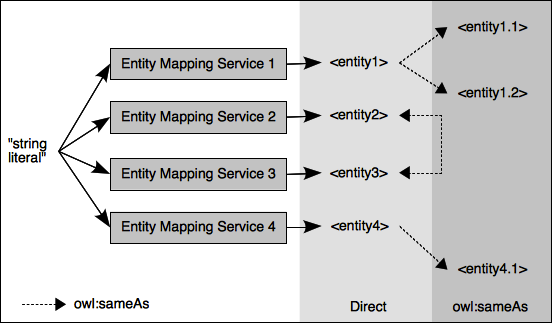
\includegraphics[width=0.8\textwidth]{diagram.png}
 \caption{Exemplary result set configuration using four entity mapping services with only the particular top result displayed for each entity mapping service. The figure shows the direct results of the particular entity mapping service, and \texttt{owl:sameAs} results for the direct results.}
 \label{fig:diagram}
\end{figure*}

In the following we will discuss some strategies in order to decide for the most probable entity candidate from a given
result set configuration.

\subsection{Direct Approaches}

The most obvious class of approaches is what we call direct approaches, i.e., with direct approaches we do not look at potential \texttt{owl:sameAs} data at all, but exclusively work with the direct output of the entity mapping Web services. If in the following we talk about votes, we mean that a certain entity $x_n$ is in the considered result set of an entity mapping service for a string literal $s$.

\subsubsection{Majority-based Winner Entity Determination}\label{sec:direct}

By \textit{majority-based} we mean that simply the entity with the most votes is elected the winner entity. If no
winner can be determined, we can either randomly select a winner, or rank the candidates by the trustworthiness of the
particular Linked Data sources (a complete definition of \textit{trustworthiness of Linked Data sources} is out of
scope of this paper, however, something like the number of inbound links in the Linked Open Data
cloud\footnote{\url{http://lod-cloud.net/}} could be taken as a ranking criteria, somewhat similar to PageRank).

We can treat each of the first $n$ results of each service equally, and elect the winner entity by determining the
absolute majority of entities as in \ref{sec:direct}. The chance to have a correct entity within all results is
obviously higher the more results we consider. An obvious next step different from treating each of the first $n$
results equally would be to preserve the information of the entity mapping services' ranking by introducing rank
weights. The particular ranking formula of each entity mapping service is not necessarily known, however, we assume
that they were chosen to the best of the services' implementors' knowledge with the intention of fair ranking.

\subsubsection{Direct Source-weighted Winner Entity Determination}

Another option is to always select the trustworthiest result by the inbound links ranking criteria as outlined in the
previous section \ref{sec:direct}, independent from the majority constellation. Practically speaking this means that
if, e.g., DBpedia were considered trustworthier as, e.g.,  GeoNames\footnote{\url{http://www.geonames.org/}}, we would
trust  the DBpedia result over any other result from GeoNames.

\subsubsection{Direct Majority-based Source-weighted Winner Entity Determination}

Based on direct majority-based winner entity determination we can introduce weight factors that give trustworthy
sources a boost. This means that even if a certain trustworthy source did not have the majority of votes, it still
could win the election and be the winning entity. Obviously the final result depends on the to-be- determined concrete
weight factors and on the particular majority constellation. Conflicts can be resolved as outlined in \ref{sec:direct}.

\subsection{owl:sameAs Approaches}

With \texttt{owl:sameAs} we mean that in addition to the direct results of the entity mapping Web services we also
consider \texttt{owl:sameAs} data for the direct results.

\subsubsection{owl:sameAs Majority-based Winner Entity Determination}\label{sec:owlsameas}

Analogue to direct majority-based winner entity determination, \texttt{owl:sameAs} majority-based winner entity
determination works by introducing entity clusters. An entity cluster is defined by a direct result and its
\texttt{owl:sameAs} corresponding sub-results. The entity cluster with the most votes is then elected as winning
cluster, i.e., the winner entity is the direct result of its particular winning entity cluster.

\subsubsection{owl:sameAs Source-weighted Winner Entity Determination}

This approach is very similar to the corresponding direct approach, with the difference that a low-weight direct result
(direct in the sense of being a direct output of the entity mapping Web service) can still win if it has high-weight
\texttt{owl:sameAs} sub-results.

\subsubsection{owl:sameAs Source-weighted Majority-based Winner Entity Determination}

Within entity clusters we can apply source weights in order to emphasize trustworthy sources and then apply
majority-based winner determination as in \ref{sec:owlsameas}.

\section{Entity Consolidation}                                              \label{sec:consolidation}
We define the process of entity consolidation as the merge of entities, i.e., if several services extract the same
entity from the same input text fragment or term, we say that the entity is consolidated.

%%%  3.1 Interplay Of the Web Services  %%%
\subsection{Interplay Of the Web Services}                                  \label{sec:interplay}
As outlined before, the metadata for a YouTube video are its \textit{title}, its \textit{description}, its \textit{tags}, and its \textit{closed captions
tracks}. We first analyze the tags one-by-one with each URI lookup Web services through a helper wrapper sub-service of our Web service. We then
analyze the title combined with the description (first run) and the closed captions track (second run) through another wrapper helper sub-service with each of the NLP Web services. We have chosen this order because we have observed that sometimes video description
and closed captions are not related at all. This happens when the video description gets used not in a way to describe
the video content on a high level but, for example, to advertise different videos from the same user. In this case, the
NLP gets steered in a completely wrong direction. During our experiments, this occurred often enough for us to separate
the NLP analysis of descriptions and closed captions into two independent steps. When all these analysis steps are completed,
we try to match the extracted entities from all classes of services back in the video. In the following, we present our
approach for how to consolidate entities from URI lookup Web services and NLP Web services.

%%%  3.2 Entity Consolidation for URI Lookup Web Services  %%%
\subsection{Entity Consolidation for URI Lookup Web Services}               \label{sec:consolidation-uri}
As as first step, we have implemented a wrapper helper sub-service for all four URI lookup services (see~\ref{sec:urilookup}) that assimilates the particular
service's output to a common output format. This format is the least common multiple of the information of all Web
service results. For our experiments, we agreed on the JSON format. In the example below, we use the term ``Google
Translate'' to illustrate the approach. Three services return back a DBpedia URI, Sindice being the only one returning
a different result in a first place.
\begin{lstlisting}
[
  {
    "name": "Google Translate",
    "uris": [
      "http://dbpedia.org/resource/Google_Translate"
    ],
    "source": "freebase,uberblic,dbpedia",
    "relevance": 0.75
  }
]
\end{lstlisting}

The corresponding request to our wrapper API that calls all four URI lookup Web services in the background is via
\texttt{GET}
\url{/uri-lookup/combined/Google%20Translate} while the particular results from each service are available at
\url{/uri-lookup/{service_name}/Google%20Translate}.
We observe in this example that even in the lowest data representation level (JSON), we maintain provenance metadata in
the form of a \texttt{source} field.

In order to agree on a winner entity, a majority-based voting system is used. As soon as for two entities only one of
these entities' URIs match, we consider the entity consolidated and can merge the results. The problem, however, is
that both Freebase and Uberblic return results in their own namespaces (e.g., for ``Google Translate'' the results
are\nofootnote{\url{http://freebase.com/en/google_translate}},
and\nofootnote{\url{http://uberblic.org/resource/67dc7037-6ae9-406c-86ce-997b905badc8#thing}}), whereas Sindice and
DBpedia Lookup return results from DBpedia (Sindice returns other results as well). Freebase and Uberblic interlink
their results with DBpedia at an \url{owl:sameAs} level in the case of Freebase, and by referencing the source
(\url{umeta:source_uri}) for Uberblic. Therefore, by retrieving and parsing the referenced resources in the services'
namespaces, we can map back to DBpedia URIs and thus match all four services' results on the DBpedia level. Each
service's result contributes with a relevance of 0.25 to the final result. In this example, when three services agree
on the same result, the resulting relevance is thus the sum of the singular relevance scores (0.75 in this case).

%%%  3.3 Entitiy Consolidation for NLP Web Services  %%%
\subsection{Entitiy Consolidation for NLP Web Services}                     \label{sec:consolidation-nlp}
Similarly to URI lookup entity consolidation, we have implemented a second wrapper helper Web service for the three NLP services (see~\ref{sec:nlp}). While the
original calls to each particular NLP service are all HTTP \texttt{POST}-based, we have implemented the wrapper
\texttt{GET}- and \texttt{POST}-based. All NLP Web services return entities with their types and/or subtypes, names,
relevance, and URIs that link into the LOD cloud. The problem is that each service has implemented its own typing
system and providing mappings for all of them would be a relatively time-consuming task. However, as all services
provide links into the LOD cloud, the desired typing information can be pulled from there in a true Linked Data manner. The least common
multiple of the results for the query ``Google Translate'' is depicted below. For the sake of clarity, we just show one
entity with two URIs while the original result contained seven entities among which six were relevant and one was just
related.
\begin{lstlisting}
[
  {
    "name": "Google Translate",
    "relevance": 0.7128319999999999,
    "uris": [
      {
        "uri": "http://dbpedia.org/resource/Google_Translate",
        "source": "alchemyapi"
      },
      {
        "uri": "http://rdf.freebase.com/ns/en/google_translate",
        "source": "zemanta"
      }
    ],
    "source": "alchemyapi,zemanta"
  }
]
\end{lstlisting}

These results come from a request to our wrapper API via \texttt{GET} \url{/entity-extraction/combined/Google%20Translate},
and similarly to the URI lookup, the particular services' results can be obtained at \url{/entity-extraction/{service_name}/Google%20Translate%20is%20a%20service%20by%20Google}.
While AlchemyAPI and Zemanta return results from DBpedia and other interlinked LOD cloud resources, OpenCalais returns
only results in its own namespace
(e.g.\nofootnote{\url{http://d.opencalais.com/er/company/ralg-tr1r/ce181d44-1915-3387-83da-0dc4ec01c6da.rdf}} for the
company Google). In this particular case, retrieving the resource RDF representation and parsing for
\texttt{owl:sameAs} return links to DBpedia. However, in the general case, we found OpenCalais URIs sometimes pointing
to non-existent resources or to not very rich resources such
as\nofootnote{\url{http://d.opencalais.com/pershash-1/cfcf1aa2-de05-3939-a7d5-10c9c7b3e87b.html}}, a URI identifying
the current US President Barack Obama where the only information is that Barack Obama is of type person. In order to
consolidate extracted entities, we use the following approach: we have a look at each of the extracted entities from
service one and compare each entity's URIs with each URIs from each extracted entity from service two. The examples
below illustrate this process.

First, we consider the isolated results for the text fragment from AlchemyAPI only:
\begin{lstlisting}
{
  "name": "Google",
  "relevance": 0.496061,
  "uris": [
    {
      "uri": "http://dbpedia.org/resource/Google",
      "source": "alchemyapi"
    },
    {
      "uri": "http://rdf.freebase.com/ns/guid.9202a8c04000641f800000000042acea",
      "source": "alchemyapi"
    },
    {
      "uri": "http://cb.semsol.org/company/google.rdf",
      "source": "alchemyapi"
    }
  ],
  "source": "alchemyapi"
}
\end{lstlisting}

Second, we consider the isolated results for the same text fragment from Zemanta only:
\begin{lstlisting}
{
  "name": "Google Inc.",
  "relevance": 0.563132,
  "uris": [
    {
      "uri": "http://rdf.freebase.com/ns/en/google",
      "source": "zemanta"
    },
    {
      "uri": "http://dbpedia.org/resource/Google",
      "source": "zemanta"
    },
    {
      "uri": "http://cb.semsol.org/company/google#self",
      "source": "zemanta"
    }
  ],
  "source": "zemanta"
}
\end{lstlisting}

Finally, we consider the merged results from both Zemanta and AlchemyAPI. Note that these results are not exposed externally, they are used internally by the wrapper helper Web service:
\begin{lstlisting}
{
  "name": [
    "Google",
    "Google Inc."
  ],
  "relevance":  0.5295965,
  "uris": [
    {
      "uri": "http://dbpedia.org/resource/Google",
      "source": "alchemyapi"
    },
    {
      "uri": "http://rdf.freebase.com/ns/guid.9202a8c04000641f800000000042acea",
      "source": "alchemyapi"
    },
    {
      "uri": "http://umbel.org/umbel/ne/wikipedia/Google",
      "source": "alchemyapi"
    },
    {
      "uri": "http://cb.semsol.org/company/google.rdf",
      "source": "alchemyapi"
    },
    {
      "uri": "http://rdf.freebase.com/ns/en/google",
      "source": "zemanta"
    },
    {
      "uri": "http://cb.semsol.org/company/google#self",
      "source": "zemanta"
    }
  ],
  "source": "alchemyapi,zemanta"
}
\end{lstlisting}

In this example, the entity names mismatch (``google inc.'' vs. ``google''). However, going down the list of URIs for
the entity, one can note a match via\nofootnote{\url{http://dbpedia.org/resource/Google}}. Additionally, one can also
see two would-be matches: \nofootnote{\url{http://cb.semsol.org/company/google.rdf}}
vs.\nofootnote{\url{http://cb.semsol.org/company/google#self}} and
\nofootnote{\url{http://rdf.freebase.com/ns/en/google}} vs.
\nofootnote{\url{http://rdf.freebase.com/ns/guid.9202a8c04000641f800000000042acea}}. However, the inconsistent use of
URIs when there is more than one URI available for the same entity hinders the match from being made. An additional
retrieval of the resources would be necessary to detect that in the latter case
\nofootnote{\url{http://rdf.freebase.com/ns/guid.9202a8c04000641f800000000042acea}} redirects to
\nofootnote{\url{http://rdf.freebase.com/ns/en/google}}, whereas the first example seems to be broken
(\nofootnote{\url{http://cb.semsol.org/company/google#self}} returns the status code 404). The good thing, however, is
that as soon as one match has been detected, one can consolidate the entities from both services.

Given the mismatching two entity names (``google inc.'' vs. ``google''), the consolidated name is then an array of all
detected synonymous. The consolidated relevance is the average relevance of both services. In contrast to URI lookup
where we had to manually assign a relevance of 0.25 to each result since not all URI lookup services include the
concept of relevance in their results, with NLP services, each service already includes a relevance score ranging from
0 (irrelevant) to 1 (relevant), so we can directly use it. In our approach, the consolidated and merged entities from
service one and two are then in turn compared to extracted entities from service three and so on, if we used even more
services. In practice, however, due to the not always given interconnectedness of OpenCalais, there are no matches
after having compared Zemanta-extracted entities with AlchemyAPI-extracted entities. Similarly to URI lookup-detected
entity consolidation, we also maintain provenance metadata for each URI on the lowest data representation level (JSON)
on both a per URI basis and an entity basis with the NLP-detected entity consolidation.

We note that in our example, the results from URI lookup are a subset of the results from NLP. However, while all URI
Lookup services accept one-word arguments (e.g., ``google''), only AlchemyAPI from the NLP services accepts one-word
arguments. The two other services accept only non-trivial text fragments (e.g., ``google is a company founded by larry
page'').

%%%  3.4 Identity Links On the Semantic Web  %%%
\subsection{Identity Links On the Semantic Web}                             \label{sec:sameasorg}
In order to tackle the problem of different namespaces in results that we have outlined in the
Section~\ref{sec:consolidation-uri}, a straightforward idea is to use a Web service such as
<sameAs>\footnote{\url{http://sameas.org/}} to easily find mappings from one namespace into another. In practice,
however, while many data sources in the Linked Data world are marked as being equal to each other (e.g.,
\url{http://dbpedia.org/resource/Barack_Obama} \texttt{owl:sameAs} \url{http://rdf.freebase.com/rdf/en.barack_obama}),
the quality of such equality links is not always excellent. As Halpin et al. show in~\cite{Halpin:SameAs}, the problem
with \texttt{owl:sameAs} is that people tend to use it very differently. The authors of~\cite{Halpin:SameAs}
differentiate four separate usage styles, each with its particular implications. Inference is thus problematic, if not
impossible, when the sense of the particular use of \texttt{owl:sameAs} is unknown.

\section{Structuring Unstructured Data}    \label{sec:services}
Sir Tim Berners-Lee has introduced Linked Data in a W3C Design Issue~\cite{TimBL:LinkedData}, where he defines the four rules for Linked~Data:
\begin{enumerate}
\item Use URIs as names for things.
\item Use HTTP URIs so that people can look up those names.
\item When someone looks up a URI, provide useful information, using the standards (RDF*, SPARQL).
\item Include links to other URIs, so that they can discover more things.
\end{enumerate}
In order to represent extracted named entities from Facebook microposts in an unambiguous way, we apply the first and the second Linked Data principle by representing named entities with HTTP URIs. This is taken care of by the third party NLP APIs that we use for our Chrome extension, namely OpenCalais~\cite{OpenCalais}, Zemanta~\cite{Zemanta}, DBpedia Spotlight~\cite{Spotlight}, and AlchemyAPI~\cite{AlchemyApi}. These APIs take a text fragment as input, perform named entity extraction on it, and then link the extracted entities back into the Linking Open Data (LOD) cloud\footnote{\texttt{http://lod-cloud.net/}}. We use these APIs in parallel, and by combining their results aiming at the emergence effect in the sense of Aristotle: ``\emph{[\ldots] the totality is not, as it were, a mere heap, but the whole is something besides the parts [\ldots]}''\footnote{Aristotle, Metaphysics, Book H 1045a 8-10.}. 

\subsection{Combining Results from Different NLP APIs}                     \label{sec:consolidation-nlp}
We have implemented a mash-up API for the four NLP APIs. While the original calls to each particular NLP API are all HTTP \texttt{POST}-based, we have implemented a \texttt{GET}- and \texttt{POST}-based mash-up API. All NLP APIs return entities with their types and/or subtypes, names, relevance, and URIs that link into the LOD cloud. Our mash-up API supports two output formats, namely application/json and text/turtle (an RDF~\cite{RDF} serialization format). The combined output in JSON form for the micropost \emph{``Tom has the LaTeX, BibTeX, LaTeX, LaTeX blues...''} (see Figure~\ref{fig:facebook}) is shown below:
\begin{lstlisting}
[
  {
    "name": "LaTeX",
    "relevance": 0.7128319999999999,
    "uris": [
      {
        "uri": "http://dbpedia.org/resource/LaTeX",
        "source": "zemanta"
      }
    ],
    "source": "zemanta"
  },
  {
    "name": "BibTeX",
    "relevance": 0.8143277777777777,
    "uris": [
      {
        "uri": "http://dbpedia.org/resource/BibTeX",
        "source": "zemanta"
      }
    ],
    "source": "zemanta"
  }  
]
\end{lstlisting}

These joint results come from a request to our mash-up API via \texttt{GET} \texttt{/entity-extraction/combined/Tom\%20has\%20\-the\%20LaTeX\%2C\%20BibTeX\%2C\%20\-LaTeX\%2C\%20LaTeX\%20blues...}. Obviously our API abstracts away the different output formats of the underlying APIs and returns a JSON object structure instead.

\subsection{The Need for Providing Provenance Metadata}
Hartig et al. mention in~\cite{ipaw10:olaf} some reasons that justify the need for provenance metadata. Among those is linked dataset replication and distribution on the Web with not necessarily identical namespaces: based on the same source data, different copies of a linked dataset can be created with different degrees of interconnectedness by different publishers.

We add to this list the automatic conversion of legacy unstructured data to Linked Data with heuristics where extracted entities -- while being consolidated and backed up by different data sources -- might still be wrong. Especially with our ``mash-up''-like approach, it is very desirable to be able to track back to the concrete source where a certain piece of information comes from. This enables (i) to correct the error at the root of our API (fighting the cause), (ii) to correct the concrete error in an RDF annotation (fighting the symptom), and (iii) to judge the trustworthiness and quality of a dataset, which is probably the most important reason.

\section{Tracking Provenance With Multiple Sources}                    \label{sec:tracking}
As outlined before, we use several data sources (APIs) in the background in order to add meaning to Facebook microposts. Extracted named entities from a Facebook micropost might in consequence be the result of up to four agreeing (or disagreeing) API calls (see Section~\ref{sec:services}). In order to track the contributions of the various sources, we have decided to use the Provenance Vocabulary~\cite{Hartig:Provenance} by Hartig and Zhao with the prefix \texttt{prv}, the HTTP Vocabulary in RDF~\cite{HTTP:RDF} by Koch et al. with prefix \texttt{http}, and a vocabulary for Representing Content in RDF~\cite{CNT:RDF} by the same authors with prefix \texttt{cnt}. We have chosen the HTTP Vocabulary in RDF for the fact that it is a W3C Working Draft  developed by the Evaluation and Repair Tools Working Group (ERT WG), which is part of the World Wide Web Consortium (W3C) Web Accessibility Initiative (WAI). The Provenance Vocabulary was chosen because of its relatively broad implementation in several projects, such as Pubby\footnote{\texttt{http://www4.wiwiss.fu-berlin.de/pubby/}}, Triplify\footnote{\texttt{http://triplify.org/Overview}}, and D2R Server\footnote{\texttt{http://www4.wiwiss.fu-berlin.de/bizer/d2r-server/}}.

While our mash-up API supports two output formats (application/json and text/turtle), we have added provenance information exclusively to the text/turtle variant. In order to represent the extracted named entities in a Facebook micropost, we use the Common Tag vocabulary~\cite{CommonTag:Spec}. A micropost is \texttt{ctag:tagged} with a \texttt{ctag:Tag}, which consists of a textual \texttt{ctag:label} and a pointer to a resource that specifies what the label \texttt{ctag:means}. The Common Tag vocabulary is well-established and developed by both industry and academic partners. In order to make statements about a bundle of triples, we group them in a named graph. We use the TriG~\cite{Bizer:TriG} syntax:
\begin{lstlisting}
:G = {
  <https://www.facebook.com/Tomayac/posts/10150175940867286> ctag:tagged [
      a ctag:Tag ;
      ctag:label "BibTeX" ;
      ctag:means <http://dbpedia.org/resource/BibTeX>
    ] .
} .
\end{lstlisting}

\subsection{The Provenance Vocabulary}                                      \label{sec:provenance}
In this section, we outline the required steps in order to make statements about the provenance of a group of triples contained in a named graph \texttt{:G} that was generated using several HTTP \texttt{GET} requests to third party APIs. We use the Provenance Vocabulary~\cite{Hartig:Provenance} with prefix \texttt{prv}, the HTTP Vocabulary in RDF~\cite{HTTP:RDF} with prefix \texttt{http}, and the Representing Content in RDF~\cite{CNT:RDF} vocabulary with prefix \texttt{cnt}.

First, we state that \emph{:G} is both a \emph{prv:DataItem} and obviously an \emph{rdfg:Graph}. \emph{:G} is \emph{prv:createdBy} the process of a \emph{prv:DataCreation}. This \emph{prv:DataCreation} is \emph{prv:performedBy} a \emph{prv:NonHumanActor}, a \emph{prvTypes:DataProvidingService} to be precise (simplified as \emph{http://tomayac.no.de/entity-extraction/combined} in the listing). This service is \emph{prv:operatedBy} a human (\texttt{http://tomayac.com/thomas\_steiner.rdf\#me}). Time is often important for provenance, so the \emph{prv:performedAt} date of the \emph{prv:DataCreation} needs to be saved. During the process of the \emph{prv:DataCreation} there are \emph{prv:usedData}, which are \emph{prv:retrievedBy} a \emph{prv:DataAcess} that is \emph{prv:performedAt} a certain time, and \emph{prv:performedBy} a non-human actor (our API) that is \emph{prv:operatedBy} a human (\texttt{http://tomayac.com/thomas\_steiner.rdf\#me}. For the \emph{prv:DataAccess} (there is one for each third party API involved), we \emph{prv:accessedService} from a \emph{prv:DataProvidingService} of which we \emph{prv:accessedResource} at a certain \emph{irw:WebResource}. Therefore, we \emph{prvTypes:exchangedHTTPMessage} which is an \emph{http:Request} using \emph{http:httpVersion} ``1.1'' and the \emph{http:methodName} ``GET''.

\subsection{Provenance RDF Overview}                                           \label{sec:appendix}
This section provides a shortened overview of the provenance RDF in Turtle syntax for a Facebook micropost tagged with the label ``BibTeX'' and the assigned
meaning \texttt{http://dbpedia.org/resource/BibTeX}. The named graph \texttt{:G} in the first part of the listing contains the absolute data (the fact that the Facebook micropost with the URI \texttt{https://www.facebook.com/Tomayac/posts/\-10150177486072286} is tagged with the label ``BibTeX'', which is represented by the HTTP URI \texttt{http://dbpedia.org/resource/BibTeX}). The second part with metadata about \texttt{:G} says that these facts were generated via two calls, one using the HTTP method \texttt{GET}, and the other \texttt{POST}:
\begin{lstlisting}
:G = {
  <https://www.facebook.com/Tomayac/posts/10150177486072286> ctag:tagged [
     a ctag:Tag ;
     ctag:label "BibTeX" ;
     ctag:means <http://dbpedia.org/resource/BibTeX> ;
  ] .
} .


:G
  a prv:DataItem ;
  a rdfg:Graph ;
  prv:createdBy [
    a prv:DataCreation ;
    prv:performedAt "2011-05-20T15:06:30Z"^^xsd:dateTime ;
    prv:performedBy <http://tomayac.no.de/entity-extraction/combined> ;
    prv:usedData [
      prv:retrievedBy [
        a prv:DataAcess ;
        prv:performedAt "2011-05-20T15:06:30Z"^^xsd:dateTime ;
        prv:performedBy <http://tomayac.no.de/entity-extraction/combined> ;
        prv:accessedService <http://spotlight.dbpedia.org/rest/annotate> ;
        prv:accessedResource <http://spotlight.dbpedia.org/rest/annotate?text=Tom%20has%20the%20LaTeX%2C%20BibTeX%2C%20LaTeX%2C%20LaTeX%20blues...&confidence=0.4&support=20> ;
        prvTypes:exchangedHTTPMessage [
          a http:Request ;
          http:httpVersion "1.1" ;
          http:methodName "GET" ;
          http:mthd <http://www.w3.org/2008/http-methods#GET> ;
        ] ;
      ] ;
    ] ;
    prv:usedData [
      prv:retrievedBy [
        a prv:DataAcess ;
        prv:performedAt "2011-05-20T15:06:41Z"^^xsd:dateTime ;
        prv:performedBy <http://tomayac.no.de/entity-extraction/combined> ;
        prv:accessedService <http://api.zemanta.com/services/rest/0.0/> ;
        prv:accessedResource <http://api.zemanta.com/services/rest/0.0/> ;
        prvTypes:exchangedHTTPMessage [
          a http:Request ;
          http:httpVersion "1.1" ;
          http:methodName "POST" ;
          http:mthd <http://www.w3.org/2008/http-methods#POST> ;
          http:headers (
            [
              http:fieldName "Content-Type" ;
              http:fieldValue "application/x-www-form-urlencoded" ;
            ]   
          )
          http:body [
            a cnt:ContentAsText ;
            cnt:characterEncoding "UTF-8" ;
            cnt:chars """method=zemanta.suggest_markup
            &api_key=Your_API_Key
            &text=Tom%20has%20the%20LaTeX%2C%20BibTeX%2C%20LaTeX%2C%20LaTeX%20blues...
            &format=json
            &return_rdf_links=1""" ;
          ] ;
        ] ;
      ] ;
    ] ;
  ] .
\end{lstlisting}

It is to be noted that statements such as in the listing above refer to the triple objects as an identifier for a Web resource (where the Web resource is a representation of the result of the API call at the time where it was \texttt{prv:performedAt}). As provenance metadata always refers to the time context in which a certain statement was made, it is essentially unimportant what representation the resource returns in future.

\section{Future Work} \label{sec:future}
Already commenced future work is to explore ways to drastically simplify the descriptions by reducing their verbosity, but still try to be compatible with existing standards such as the HTTP in RDF and Provenance vocabularies. While it is always easier to come up with a specialized vocabulary that does one task well (for example, we could imagine a simple vocabulary with the sole purpose to log the API call of an API invocation), broader reuse and acceptance can be gained by reusing existing vocabularies. We will investigate how to find the right balance here.

\section{Conclusion}                                                        \label{sec:conclusion}
We have introduced an API for adding semantic meaning to Facebook microposts. As mash-up data sources for our API we have presented NLP APIs, and then focused on the necessary RDF vocabularies to annotate Facebook microposts with the thereof extracted named entities in the form of common tags. Due to their different ``mash-up''-like history of origins, we needed to track provenance metadata in order to assure the trustworthiness of the generated data. We showed how the Provenance Vocabulary can be used to keep track of the original third party API calls that led to the consolidated results. We have shown how a concrete multi-source RESTful API can automatically maintain provenance metadata. We believe that being able to track back the origin of a piece of data is of crucial importance, however, the generated provenance-related triples are very verbose, and in consequence stating even simple facts like that a combined result is based on two separate sub-results takes up a lot of space. The verbosity is mainly due to the used vocabularies, the Provenance Vocabulary and the HTTP Vocabulary in RDF. We are conscious that our current approach is a first step in the right direction, however, that some more steps are ahead to take. Our vision is to establish a common method for specifying provenance data for mash-up APIs.

% use section* for acknowledgement
\section*{Acknowledgment}

T. Steiner is partially supported by the European Commission under Grant No. 248296 FP7 I-SEARCH project. J. Gabarr\'o is partially supported by TIN-2007-66523 (FORMALISM) and SGR 2009-2015 (ALBCOM). 

\bibliographystyle{abbrv}
\bibliography{nwesp2011}

\vspace{5mm}

\noindent{\bf\Large Author Biographies} \vspace{5mm}

\textbf{Thomas Steiner}
Thomas Steiner is a proud dad-of-two, a Research Scientist at Google, and a PhD student at UPC.edu. His main research interests these days are the Semantic Web, Linked Data, and the architectural style REST. He holds two Master of Computer Science degrees, one from the Technical University of Karlsruhe, Germany, and the other from the École Nationale Supérieure d'Informatique et de Mathématiques Appliquées de Grenoble, France. In addition to that he works on making the Internet a better place, tweets as @tomayac and blogs at blog.tomayac.com.

\vspace{4mm}

\textbf{Ruben Verborgh}
Ruben Verborgh received his Master degree in Computer Science Engineering from Ghent University, Belgium in 2010. He is a researcher with the Multimedia Lab — Ghent University, Department of Electronics and Information Systems (ELIS) and the Interdisciplinary institute for BroadBand Technology (IBBT). His interests include Semantic Web technologies, multimedia annotation, artificial intelligence, and their relation to multimedia processing. Currently, he is working on moving multimedia algorithms to the Web and associated problems, such as semantic service descriptions.

\vspace{4mm}

\textbf{Joaquim Gabarró Vallés}
Joaquim Gabarro, was born in Barcelona (Spain) in 1953 and studied Physics and Computer Science, obtained his Ph.D.
from Universitat Politècnica de Calatunya in 1983. From 1985 is Associate Professor (Profesor Titular) in Universitat Politècnica de Calatunya. Currently represents
Spain in the TC1 (Foundations of Computer Sciences) of IFIP. Main research topics
are Concurrency, Complexity and
Web algoritms.

\vspace{4mm}

\textbf{Rik Van de Walle}
Rik Van de Walle received his M.Sc. and PhD degrees in Engineering from Ghent University, Belgium in 1994 and 1998 respectively. After a visiting scholarship at the University of Arizona (Tucson, USA), he returned to Ghent University, where he became professor of multimedia systems and applications, and head of the Multimedia Lab. His current research interests include multimedia content delivery, presentation and archiving, coding and description of multimedia data, content adaptation, and interactive (mobile) multimedia applications.

\end{document}
